\documentclass{article}

\usepackage{graphicx}
\usepackage{tikz}
\usepackage{tikzsymbols}
\usetikzlibrary{calc,patterns,shapes.geometric}
\pagestyle{empty}
\usepackage[margin=0pt]{geometry}
\geometry{papersize={14in,12in}}

\def\centerarc[#1](#2)(#3:#4:#5){\draw[#1] ($(#2)+({#5*cos(#3)},{#5*sin(#3)})$) arc (#3:#4:#5);}

\begin{document}
	\begin{figure}
		\centering
		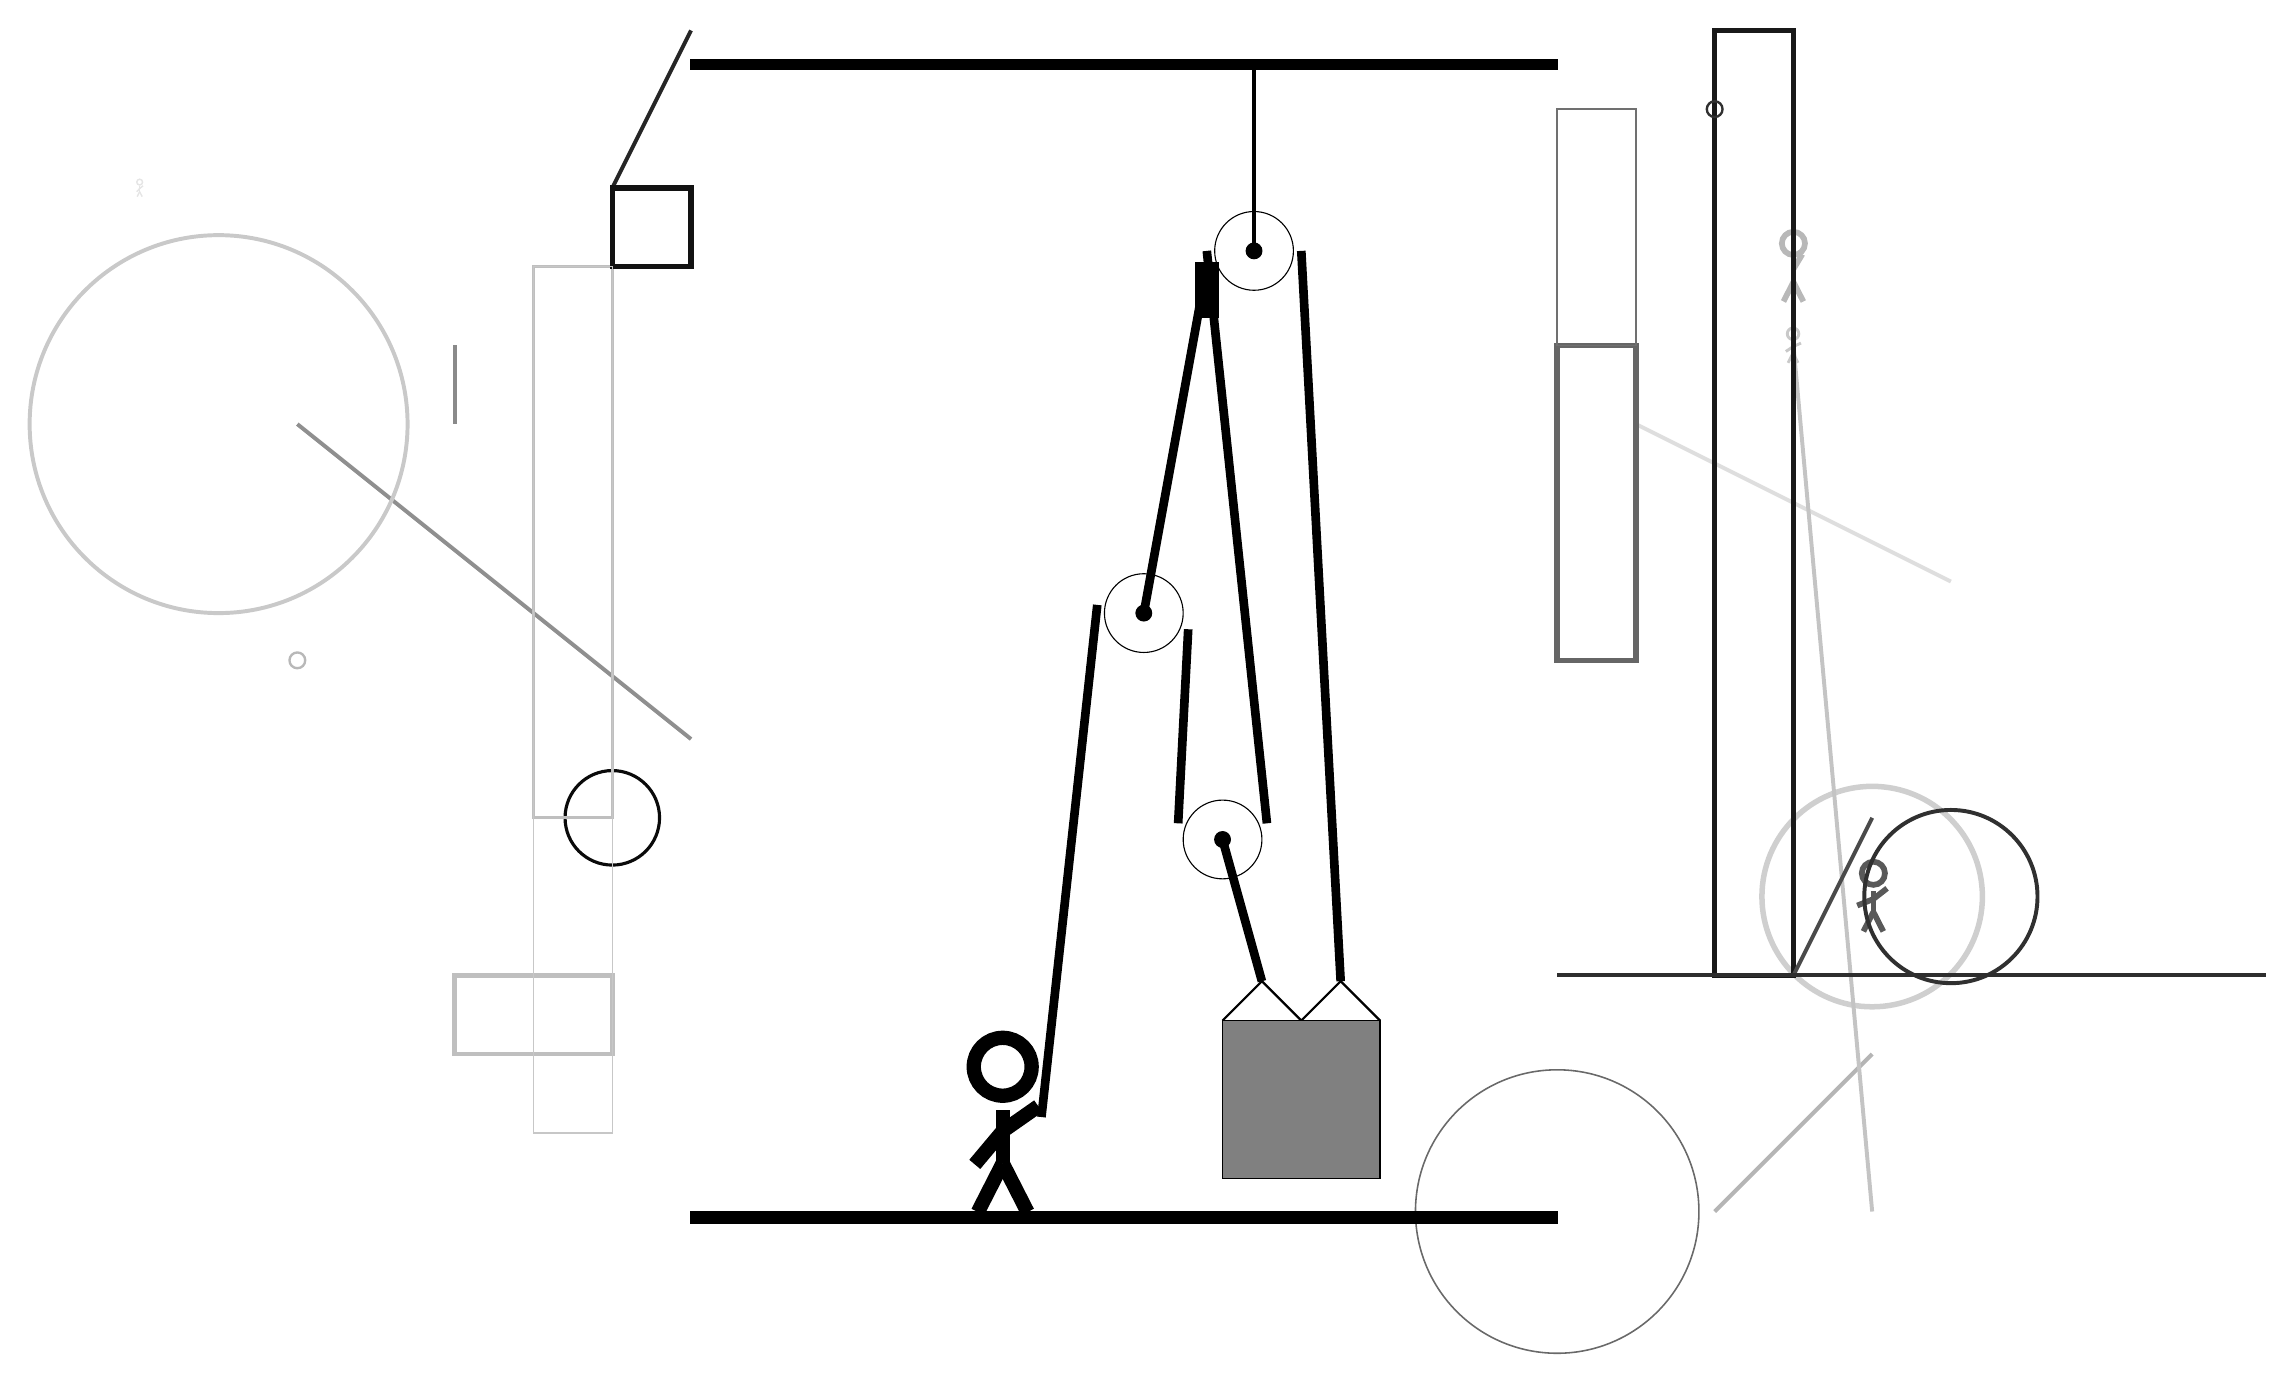
\begin{tikzpicture}
			%%%%% START %%%%%
			
			\draw[fill=black] (-6, 11.5) rectangle (5, 11.625);
			
			\draw (-0.25, 4.6) circle (0.5);
			\draw[fill=black] (-0.25, 4.6) circle (0.1);
			
			\draw (0.75, 1.725) circle (0.5);
			\draw[fill=black] (0.75, 1.725) circle (0.1);
			
			\draw (1.15, 9.2) circle (0.5);
			\draw[fill=black] (1.15, 9.2) circle (0.1);
			\draw[very thick] (1.15, 9.2) -- (1.15, 11.5);
			
			\draw[thick]  (0.75, -0.575) -- (1.25, -0.075) -- (1.75, -0.575) -- (2.25, -0.075) -- (2.75, -0.575);
			\draw[fill=black!50] (0.75, -0.575) rectangle (2.75, -2.575);
			
			\draw[line width=1.1mm] (-0.25, 4.6) -- (0.55, 9.0);
			\draw[line width=1.1mm, fill=black](0.45, 8.4) rectangle (0.65, 9.0);
			\draw[line width=1.1mm] (-1.55, -1.8) -- (-0.8409, 4.7042);
			\centerarc[line width=1.1mm](-0.25, 4.6)(-20:170:0.6);
			\draw[line width=1.1mm] (0.3138, 4.3948) -- (0.1862, 1.9302);
			\centerarc[line width=1.1mm](0.75, 1.725)(160:380:0.6);
			\draw[line width=1.1mm] (1.3138, 1.9302) -- (0.55, 9.2);
			\draw[line width=1.1mm](0.75, 1.725) -- (1.25, -0.075);
			\centerarc[line width=1.1mm](1.15, 9.2)(0:180:0.6);
			\draw[line width=1.1mm] (1.75, 9.2) -- (2.25, -0.075);
			
			\node at (-2, -1.9) {\Strichmaxerl[10][50][35]};
			
			\draw[line width=0.5mm, color=black!13](6, 7) -- (10, 5);
			
			\draw[line width=0.5mm, color=black!85](-7, 10) -- (-6, 12);
			\node[line width=0.6mm, color=black!28] at (8, 9) {\Strichmaxerl[4][90][59]};
			\node[line width=0.7mm, color=black!10] at (-13, 10) {\Strichmaxerl[1][47][39]};
			\draw[line width=0.5mm, color=black!29](9, -1) -- (7, -3);
			\draw[line width=0.7mm, color=black!60] (6, 8) rectangle (5, 4);
			\draw[line width=0.6mm, color=black!25] (-7, 0) rectangle (-9, -1);
			\node[line width=0.7mm, color=black!65] at (9, 1) {\Strichmaxerl[4][22][38]};
			\draw[line width=0.5mm, color=black!44](-11, 7) -- (-6, 3);
			\node[line width=0.5mm, color=black!21] at (8, 8) {\Strichmaxerl[2][34][24]};
			\draw [line width=0.7mm, color=black!19](9, 1) circle (1.4);
			\draw [line width=0.4mm, color=black!96](-7, 2) circle (0.6);
			\draw[line width=0.5mm, color=black!74](8, -1) -- (8, -1);
			
			\draw[line width=0.2mm, color=black!56] (6, 8) rectangle (5, 11);
			\draw [line width=0.2mm, color=black!59](5, -3) circle (1.8);
			\draw[line width=0.5mm, color=black!23](9, -3) -- (8, 8);
			\draw[line width=0.7mm, color=black!90] (7, 12) rectangle (8, 0);
			\draw[line width=0.5mm, color=black!71](8, 0) -- (9, 2);
			\draw [line width=0.5mm, color=black!81](10, 1) circle (1.1);
			
			\draw[line width=0.5mm, color=black!82](5, 0) -- (14, 0);
			\draw [line width=0.5mm, color=black!21](-12, 7) circle (2.4);
			
			\draw [line width=0.3mm, color=black!81](7, 11) circle (0.1);
			\draw[line width=0.4mm, color=black!25] (-7, 9) rectangle (-8, 2);
			\draw [line width=0.3mm, color=black!28](-11, 4) circle (0.1);
			\draw[line width=0.7mm, color=black!93] (-7, 10) rectangle (-6, 9);
			\draw[line width=0.2mm, color=black!22] (-7, 9) rectangle (-8, -2);
			
			\draw[line width=0.5mm, color=black!46](-9, 8) -- (-9, 7);
			
			\draw[fill=black] (-6, -3) rectangle (5, -3.15);
			
			%%%%% END %%%%%
		\end{tikzpicture}
	\end{figure}	
\end{document}